% This is one line latex comment.

\section{Methodology}

In this section, I introduce experiment details.
First, the setting for the measurement is shown in Section \ref{subsection:setting}.
Then the experiment procedure is introduced in Section \ref{subsection:procedure}.

\subsection{Experiment Setting}
\label{subsection:setting}

\begin{figure}[!t]
  \centering
  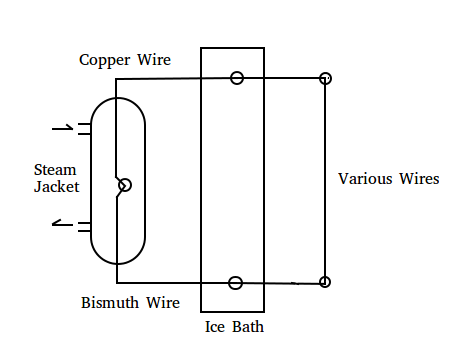
\includegraphics[width=2.5in]{setting}
  \caption{The experiment setting.}
  \label{figure:setting}
\end{figure}

Figure \ref{figure:setting} shows the setting for a series of experiments.
The left side in the figure is a thermocouple introduced in \cite{thermocouple}.
Two wires composed of two different metals, copper and bismuth, are in contact in steam jacket.
The steam jacket is used to control the heat.
By adjusting the valve, the temperature in the jacket was kept constant and under control.
At the another end of the wires, they are put into ice bath, to make the temperature difference.
The ice bath was supposed to be at 0 degree Celsius constantly.
So, by these setting, the requirements for thermocouple, which are temperature difference and the wired of different metals, was satisfied.

The right part of the Figure \ref{figure:setting} contains a setting for various wires.
To measure the effects of wire specifications, several wires with different cross-sectional area and length were connected here.
By this wire segment, the circuit is completed and finally the current becomes able to flow.

Measuring the intensity of the electrical current was accomplished by a galvanometer.
The galvanometer is placed right on the wire and measured by the angle difference the needle and the wire makes before and after the circuit is turned on.

\subsection{Experiment procedure}

